\documentclass[12pt,a4paper]{article}%
%Options -- Point size:  10pt (default), 11pt, 12pt
%        -- Paper size:  letterpaper (default), a4paper, a5paper, b5paper
%                        legalpaper, executivepaper
%        -- Orientation  (portrait is the default)
%                        landscape
%        -- Print size:  oneside (default), twoside
%        -- Quality      final(default), draft
%        -- Title page   notitlepage, titlepage(default)
%        -- Columns      onecolumn(default), twocolumn
%        -- Equation numbering (equation numbers on the right is the default)
%                        leqno
%        -- Displayed equations (centered is the default)
%                        fleqn (equations start at the same distance from the right side)
%        -- Open bibliography style (closed is the default)
%                        openbib
% For instance the command
%           \documentclass[a4paper,12pt,leqno]{article}
% ensures that the paper size is a4, the fonts are typeset at the size 12p
% and the equation numbers are on the left side
%====================Tabelas==============================================
\usepackage{multirow}
%=============================Símbolos Matemáticos=====================================================================
\usepackage{amsmath}
\usepackage{amsfonts}
\usepackage{amssymb}
\usepackage{bm} %Para Negrito no modo matematico
%=======================================Figuras===========================================================
\usepackage{graphicx}
%\usepackage{wrapfig}
\usepackage{float}
%=====================================Língua e acentos=============================================================
\usepackage[brazil]{babel}
\usepackage[utf8]{inputenc}
\usepackage[T1]{fontenc}
%========================================Espaçamento==========================================================
\usepackage[top=3cm, bottom=2cm, left=2cm, right=2cm]{geometry}
\usepackage{indentfirst}
%=======================================Lista de códigos===========================================================
\usepackage{listings}                   % para formatar código-fonte
\lstset{numbers=left, numberstyle=\tiny, stepnumber=1, numbersep=5pt, basicstyle=\scriptsize , frame=trbl}
%======================================Latexdraw============================================================
%\usepackage[usenames,dvipsnames]{pstricks}
%\usepackage{epsfig}
%\usepackage{pst-grad} % For gradients
%\usepackage{pst-plot} % For axes
%==================================================================================================
%-------------------------------------------

\begin{document}

\begin{titlepage}
\begin{center}
\begin{figure}[h]

\includegraphics[scale=0.76]{Imagens/topdotitulo.png}
\end{figure}
\rule{\columnwidth}{1.5mm}
\

\large David Maykon Krepsky Silva\\
\large Havena Louise Pavão

\vspace{4cm}
{\bf \Large Título do Experimento}
\vspace{3.5cm}

\begin{flushright}
Data de realização do experimento:\\
XX de abril de 2016\\
Série/Turma:\\
1000/1011\\
Prof. Me. Jaime Laelson Jacob 
\end{flushright}

\vspace{3.2cm}
\today

\rule{\columnwidth}{1.3mm}
\end{center}
\end{titlepage}
\newpage

\tableofcontents

\newpage

\section{Objetivo}
Revisar o uso de aplificadores operacionais, que são muito utilizados na instrumentação eletrônica.

\section{Introdução}

\subsection{Experimento 1}
Nesse experimento foi utilizado um diodo zenner como tensão de referência para a leitura de uma resistência.

\begin{figure}[H]
\begin{center}
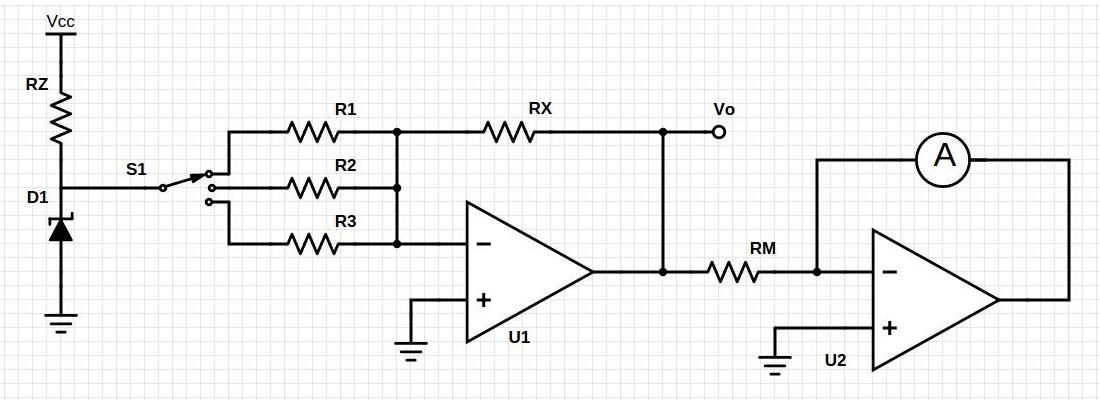
\includegraphics[scale=.25]{Imagens/cir1.jpg}
\caption{Circuito com três escalas de resistência.}
\label{cir1}
\end{center}
\end{figure}

\begin{itemize}
 \item Calcular o valor de Rz.
 \item Calcular o valor de R1, R2 e R3 de modo que fiquem três escalas distintas para a medição da resistência.
 \item Calcular o valor de Rm para limitar a corrente de acordo com a escala do amperímetro.
 \item Montar o circuito da figura 1 e utilizar 2 valores de resistência para cada escala. Medir a corrente no amperímetro e anotar os valores obtidos.
 \end{itemize} 
 
 \subsection{Experimento 2}
Neste experimento foi projetado um circuito amplificador com ganho controlado digitalmente. 
 
\begin{figure}[H]
\begin{center}
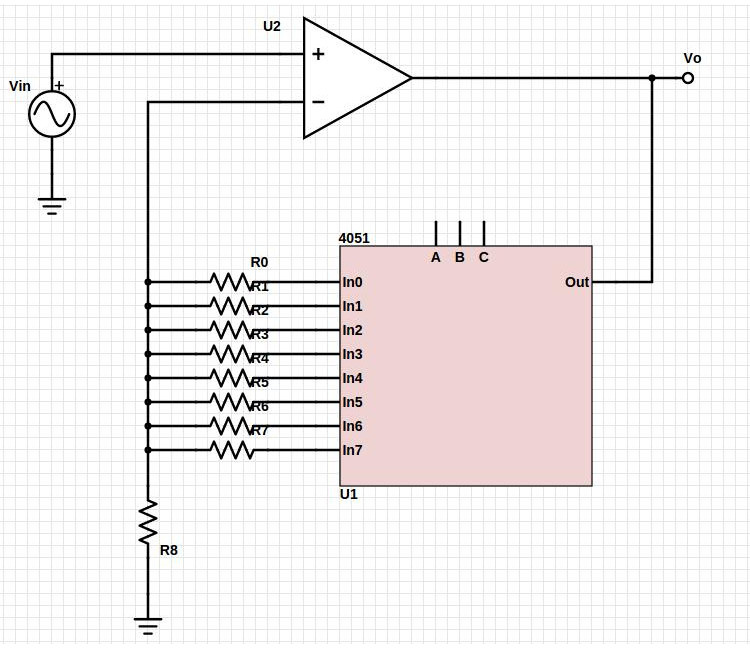
\includegraphics[scale=.3]{Imagens/cir2.jpg}
\caption{Amplificador com ganho variável.}
\label{cir2}
\end{center}
\end{figure}

\begin{itemize}
 \item Definir o valor dos resistores para 8 ganhos diferentes.
 \item Montar o circuito da \ref{cir2} e aplicar um sinal senoidal na entrada.
 \item Analizar o ganho do circuito.
 \end{itemize} 
\newpage

\section{Resultados}

\subsection{Experimento 1}
Para Rz foi considerado que o diodo D1 necessita de uma corrente de 80mA para manter a tensão estável. Sendo assim, o valor de Rz (calculado com a eq. \ref{eqRz}) foi de $108.75 \Omega$, com valor comercial mais próximo de $120 \Omega$.

\begin{equation}
Rz = \tfrac{Vcc - Vz}{80mA}
\label{eqRz}
\end{equation}

Foram definidas as escalas $1k \Omega$, $10k \Omega$  e $100k \Omega$, de modo que quando o valor de Rx for o limite da escala, a saída Vo será 10V. Os valores encontrados para os resistores R1, R2 e R3 são $330 \Omega$, $3.3k \Omega$  e  $33k \Omega$, respectivamente.

A tabela \ref{tab1} mostra o valor das resistências testadas, o valor na saída Vo e a corrente mensurada com o amperimetro.

\begin{small}
\begin{table}[H]
\begin{center}
\caption{Valores de Vo e Iout medidos.}

\begin{tabular}{l|l|l}
\hline
Rx $[\Omega]$ & Vo [V]& Iout [$\mu A$]\\
\hline
560 & 5.24 & 818\\
\hline
820 &  7.84 & 958\\
\hline
2.2k & 2.07 & 649\\
\hline
4.7k & 4.46 & 777\\
\hline
15k & 1.43 & 615\\
\hline
47k & 4.52 & 780\\
\hline

\end{tabular}
\label{tab1}
\end{center}
\end{table}
\end{small}

\subsection{Pergunta 1}
\textbf{Qual amplificador você poderia usar para reduzir erros de offset e corrente de polarização?}

Poderia ser utilizado um AmpOp de melhor qualidade, como por exemplo amplificadores operacionais feitos com JFET (TL082).

\subsection{Experimento 2}
A tabela \ref{tab2} mostra o valor das resistências escolhidas, o ganho calculado para cada resistência e o ganho medido.

O ganho calculado foi obtido através da equação do ganho para amplificadores não-inversores (eq. \ref{eq2}).

\begin{equation}
G = 1 +\tfrac{Rx}{R8}
\label{eq2}
\end{equation}

O ganho medido foi obtido aplicando-se uma entrada senoidal de frequência 1KHz e amplitude 1mV.

Foram considerados para o projeto a capacidade de \textit{sink/source} do CI 4051 e a saturação do AmpOp.

\begin{small}
\begin{table}[H]
\begin{center}
\caption{Ganho calculado e medido para cada resistor.}

\begin{tabular}{l|l|l}
\hline
Rx $[\Omega]$ & G calculado [V/V] & G medido [V/V]\\
\hline
1k & 2 & 1.7\\
\hline
4.7k &  5.7 & 5.3\\
\hline
8.2k & 9.2 & 9.0\\
\hline
22k & 23 & 22.4\\
\hline
47k & 48 & 48.0\\
\hline
100k & 101 & 100.4\\
\hline
220k & 221 & 222.0\\
\hline
470k & 471 & 469.6\\
\hline

\end{tabular}
\label{tab2}
\end{center}
\end{table}
\end{small}


\subsection{Pergunta 2}
\textbf{Que modificação poderia ser feita no circuito anterior para o ganho unitário ser possível?}

Poderia ser utilizado dois amplificadores inversores em cascata.
\newpage
\section{Anexos}

\begin{figure}[H]
\begin{center}
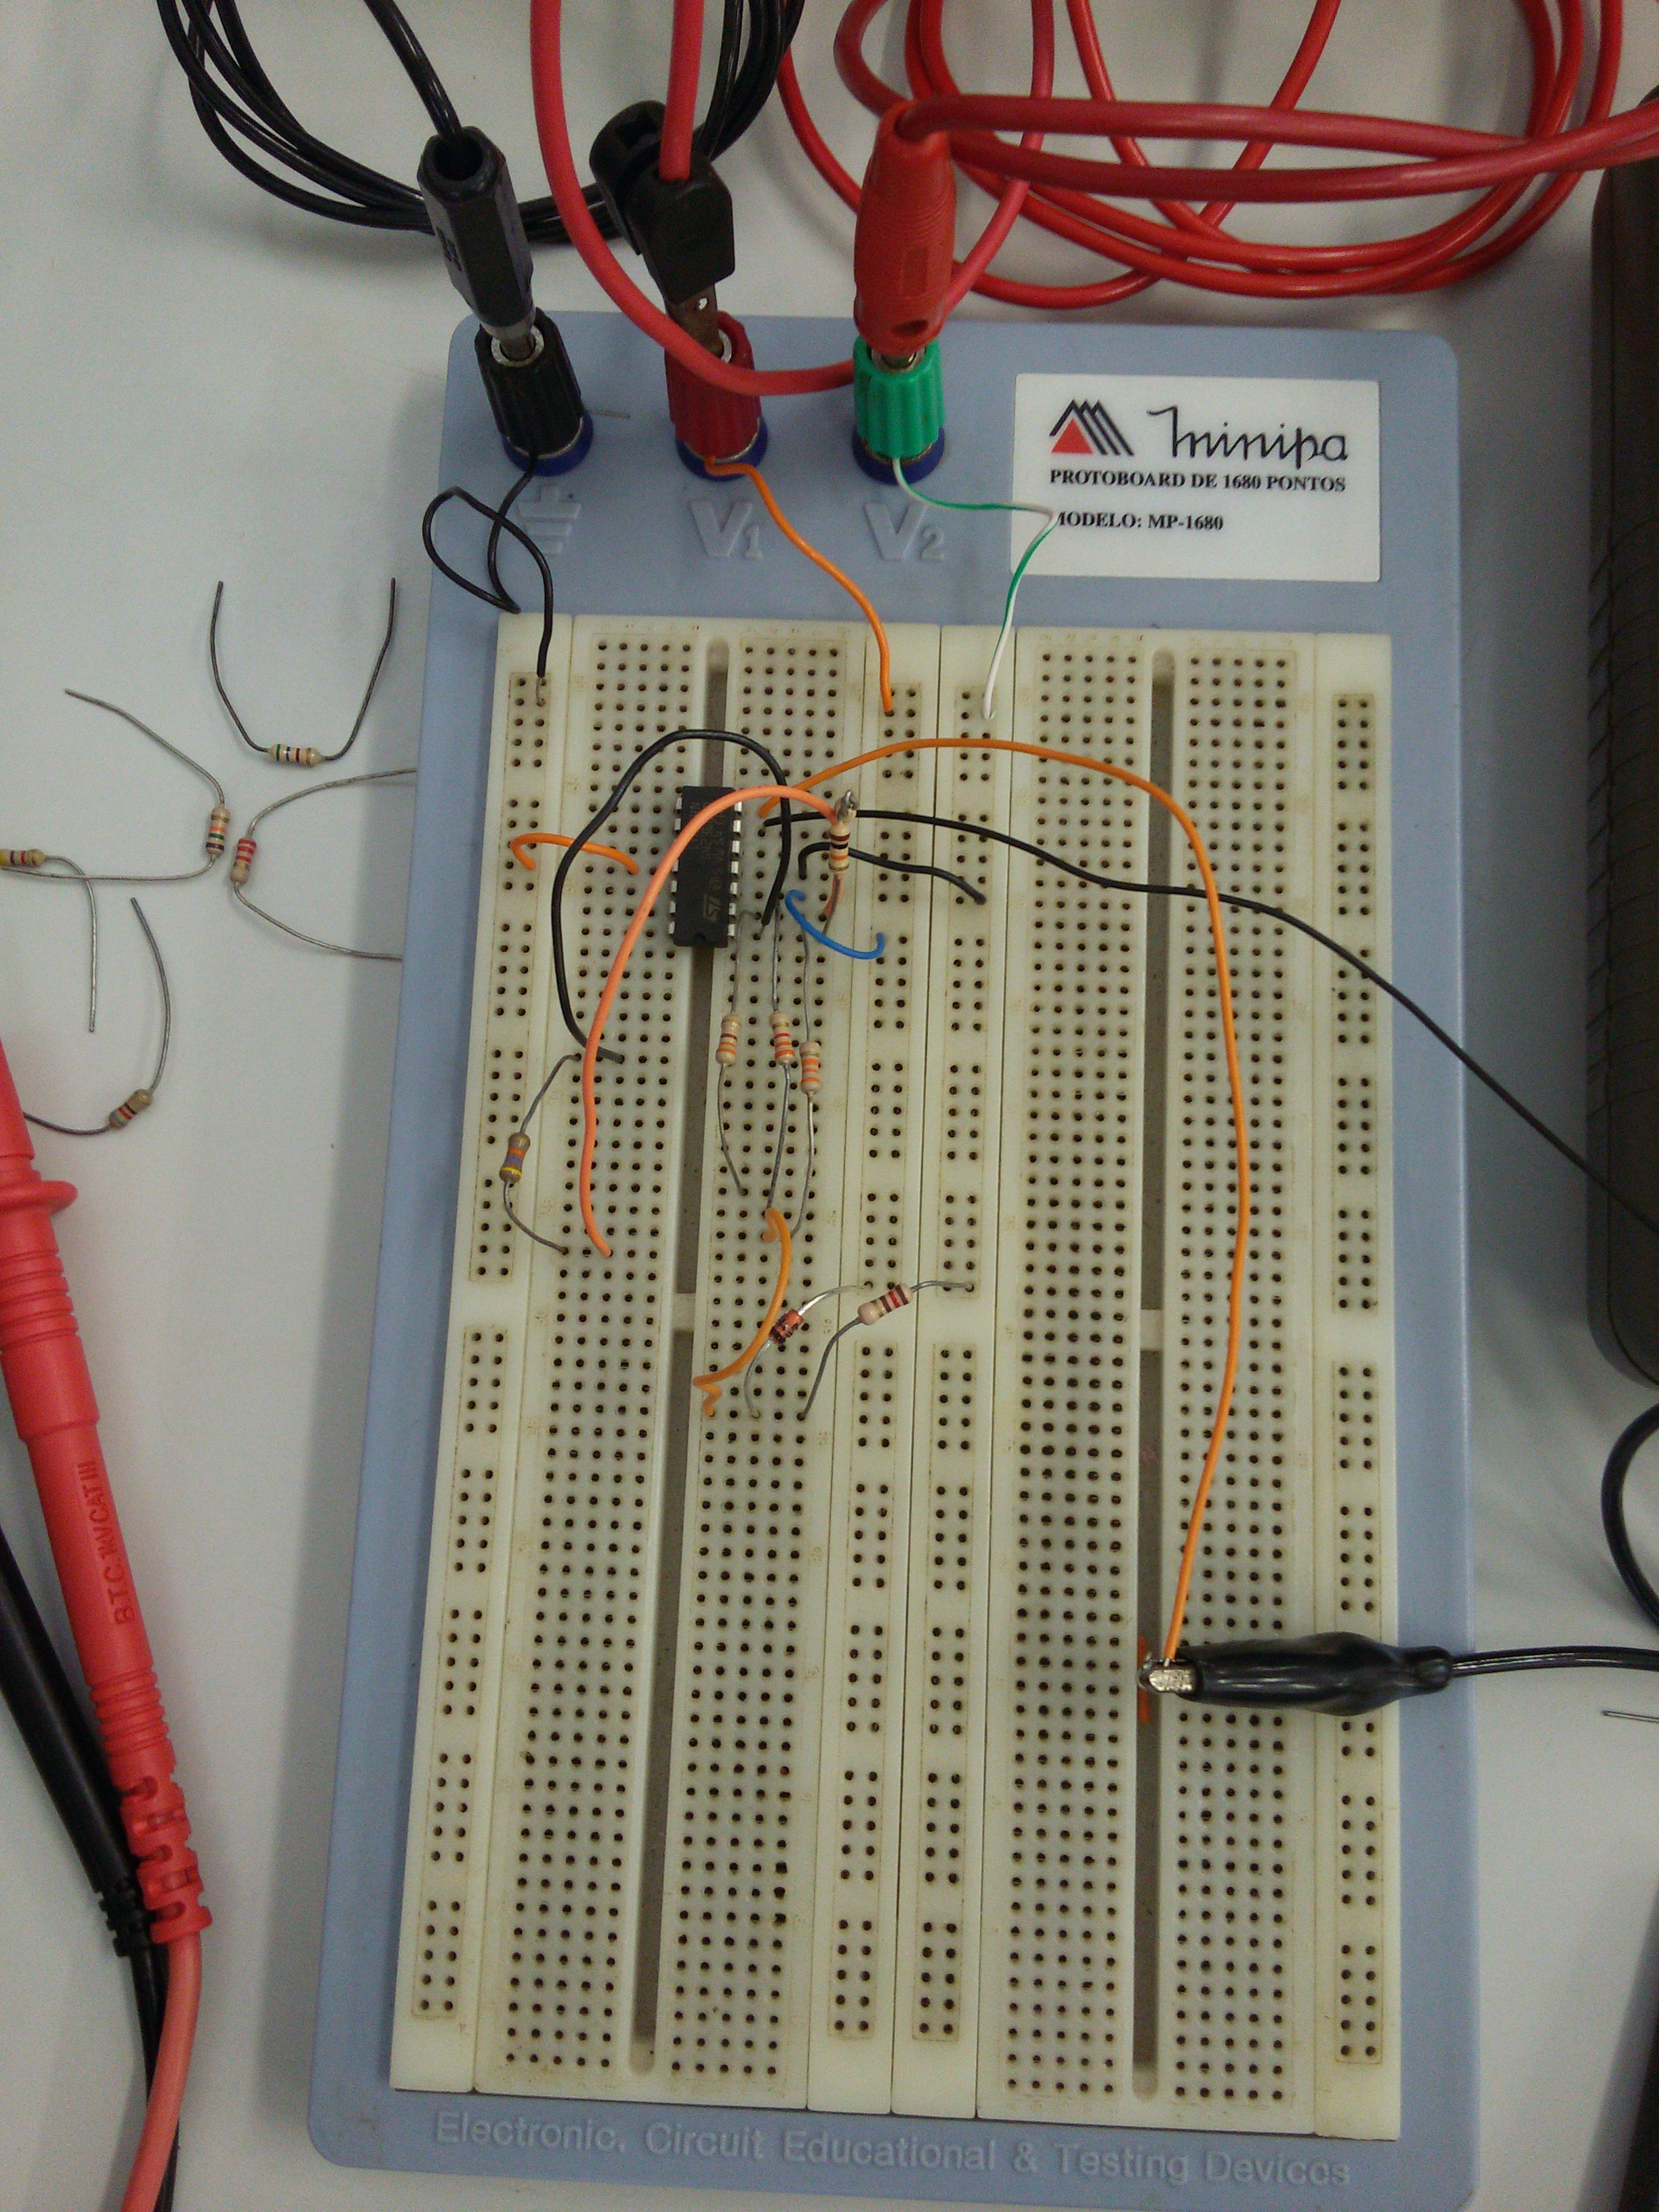
\includegraphics[scale=.1]{Imagens/exp1.jpg}
\caption{Montagem do experimento 1.}
\label{exp1}
\end{center}
\end{figure}


\begin{figure}[H]
\begin{center}
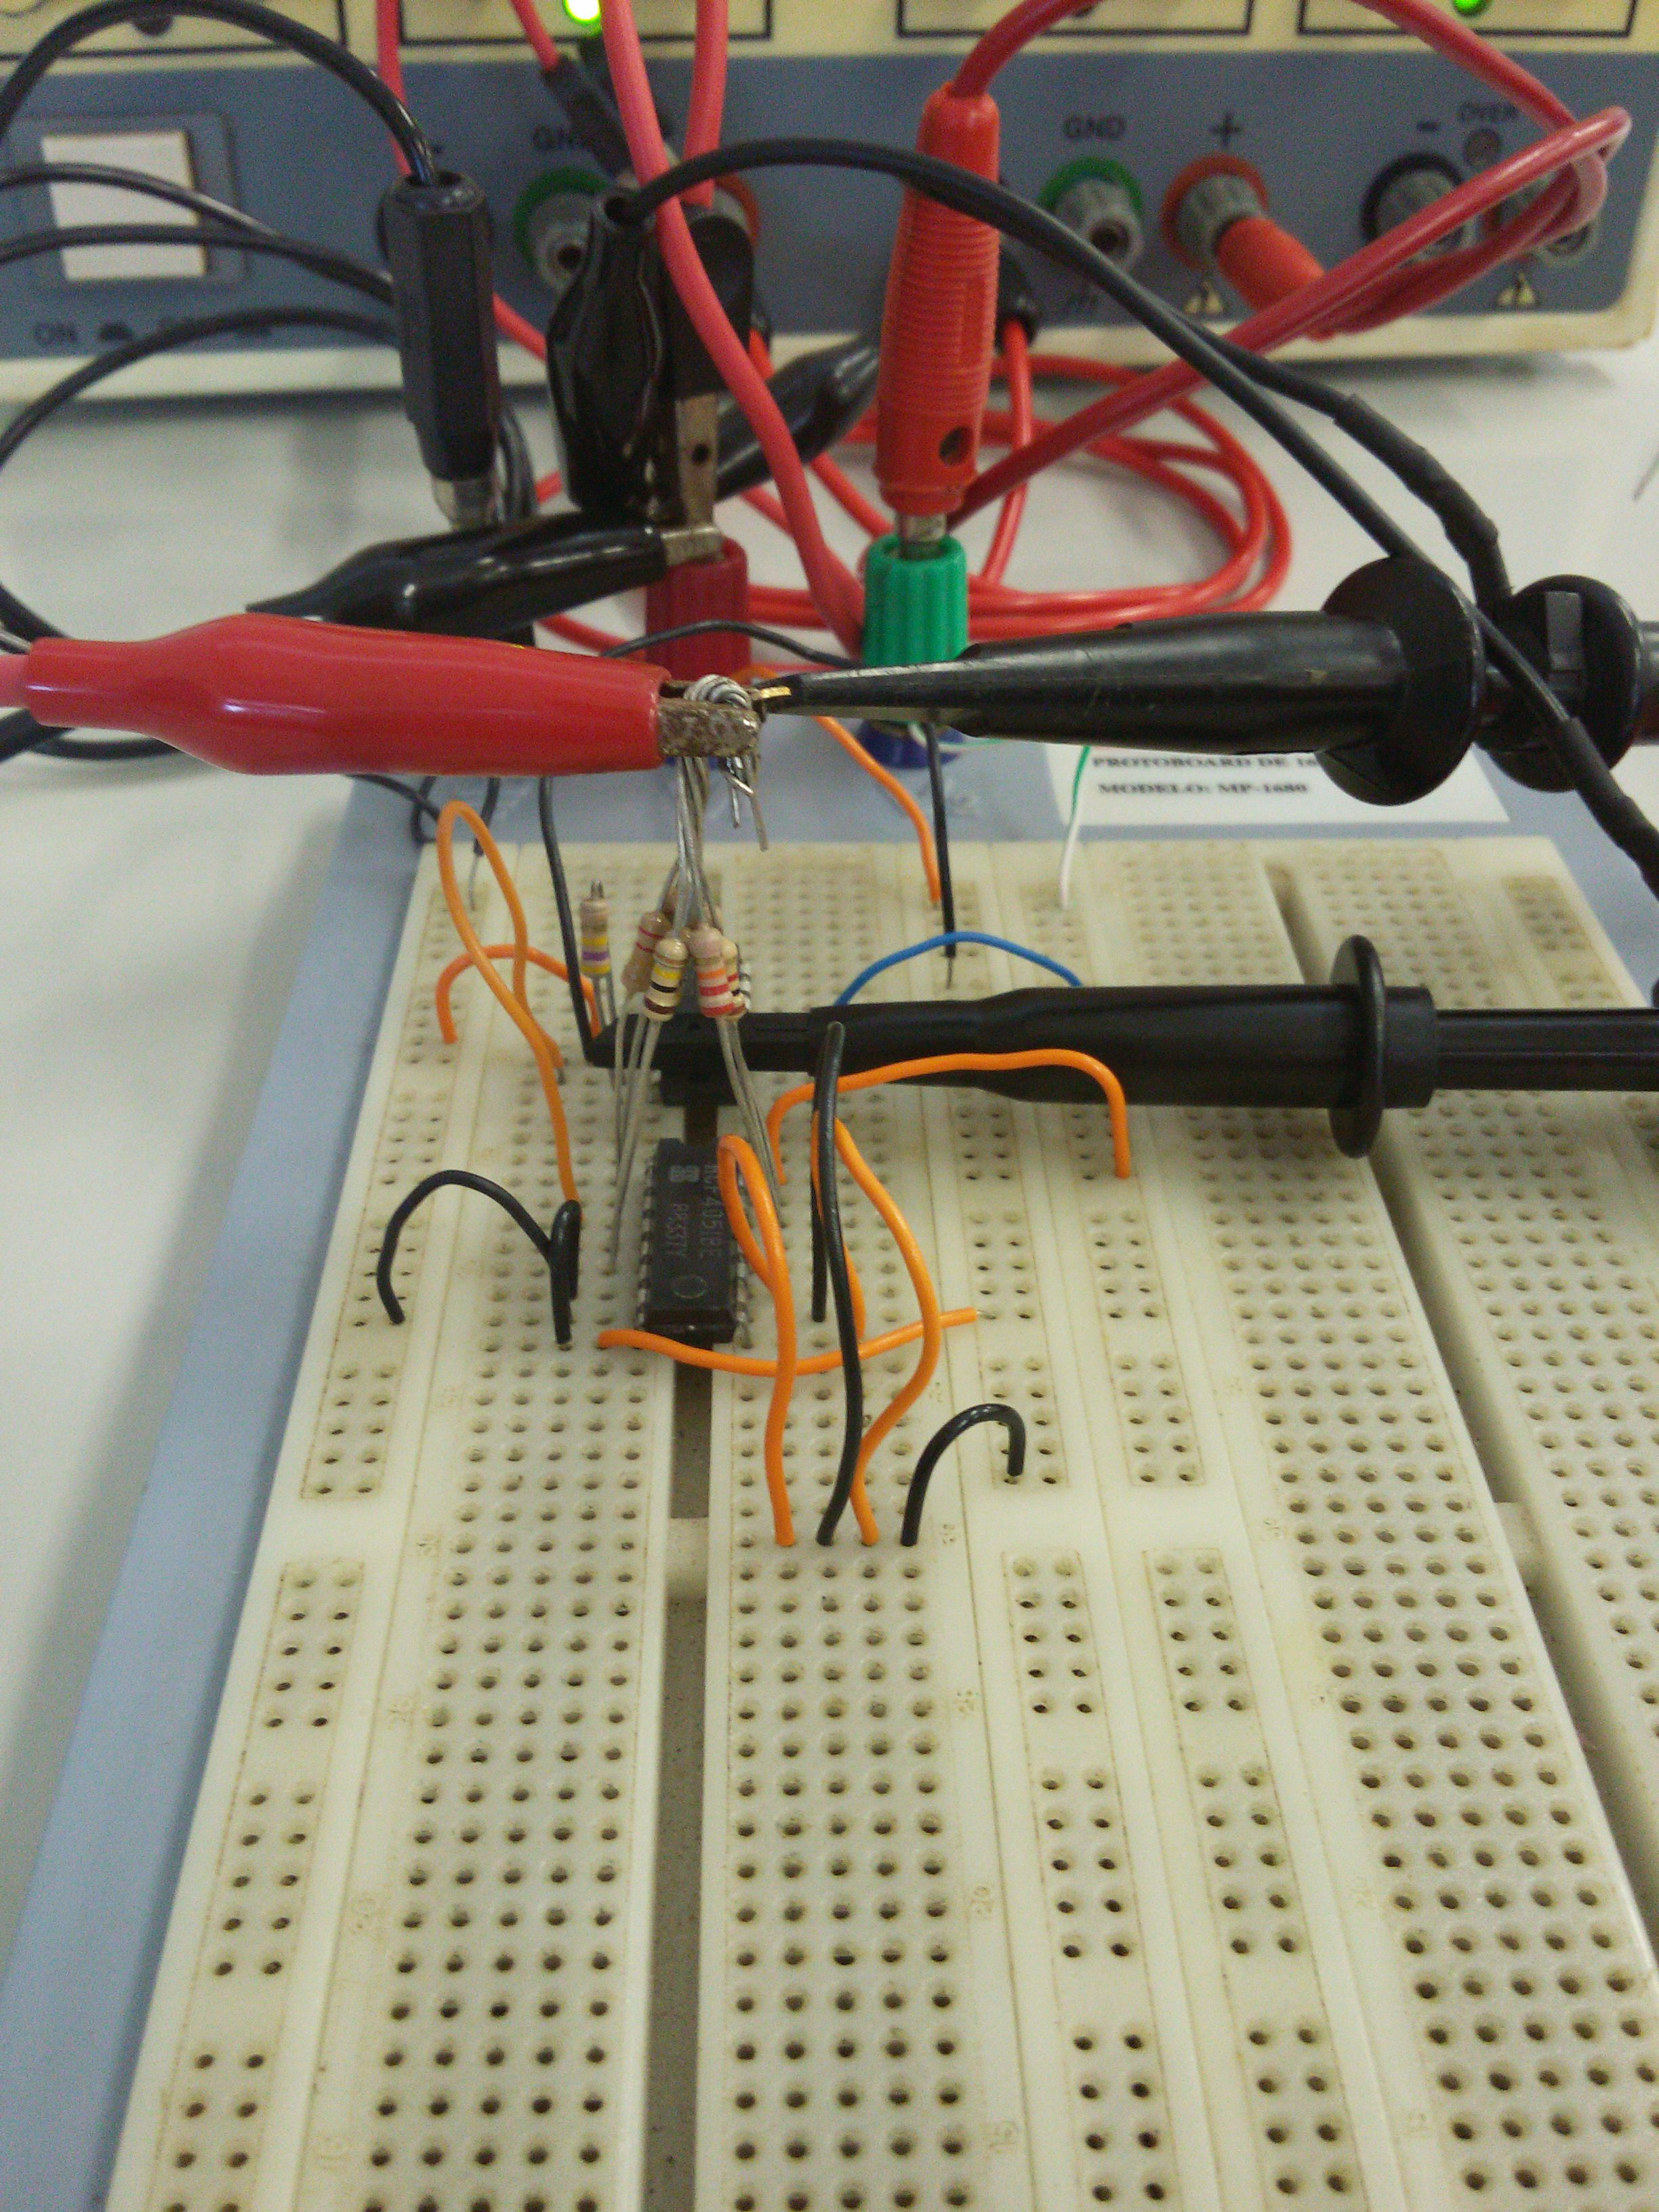
\includegraphics[scale=.1]{Imagens/exp2.jpg}
\caption{Montagem do experimento 2.}
\label{exp2}
\end{center}
\end{figure}
\end{document}